%%==================================================
%% chapter01.tex for BIT Master Thesis
%% modified by yang yating
%% version: 0.1
%% last update: Dec 25th, 2016
%%==================================================
\chapter{绪论}
\label{chap:intro}
\section{研究背景与意义}
代码克隆,也叫代码复用,是指在软件系统中存在两个或两个以上的相似代码片段\cite{乐乔艺2021代码克隆检测研究进展综述},是软件开发中的常见现象。随着互联网时代的发展,网络上各种开源项目越来越多样化,获取也更加便利。许多企业通过软件资源库、外部开源软件、软件产品线及开发框架等方式建立了多种多样的软件复用开发方法,同时开发人员自身也会通过多种方式大量复用已有的软件资源。在这些软件复用方法和资源的支持下,软件系统和软件产品大量引入了开源软件、网络资源、商业软件等第三方代码成分。这些第三方代码在多个软件系统中复制、传播和演化,给软件系统带来了软件质量的不确定性和风险,甚至导致漏洞的传播。

近年来,第三方代码中包含的漏洞数量呈现出快速增长的趋势。根据美国新思科技公司(Synopsys, Inc.)发布的《2023年开源安全和风险分析报告》\cite{Synopsys_2023}显示,在2022年审计的1703个代码库中,98\%的项目都包含开源代码,84\%的代码库包含至少一个已知开源漏洞,比2022年版的报告中增加了近4\%,有48\%代码库中包含高风险漏洞。
图\ref{fig:Proportion}统计了2018年至2022年Synopsys审计代码库中开源代码及漏洞占比,从图中可以看出开源代码及漏洞数量整体呈上升趋势。
\begin{figure}[H]
    \centering
    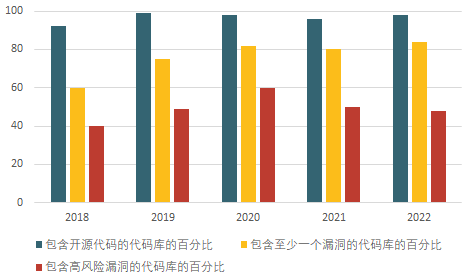
\includegraphics[width=0.75\textwidth]{figures/Proportion}
    \caption{2018-2022年Synopsys审计代码库中的开源代码及漏洞占比示意图}\label{fig:Proportion}
\end{figure}

同时,Synopsys统计了包含易受攻击组件的代码库占比,其中使用JQuery 和 Lodash 两个最流行的开源组件的代码库占比达到了47\%和 31\%,其余组件占比如图\ref{fig:assembly}所示。一旦易受攻击组件出现安全问题,通常会导致软件遭受供应链攻击。据Gartner\cite{Gartner_2022}预测,到2025年,全球45\%的组织将遭受软件供应链攻击,比2021年增加三倍。因此,准确地检测代码克隆对于软件开发和维护是至关重要的。
\begin{figure}[H]
    \centering
    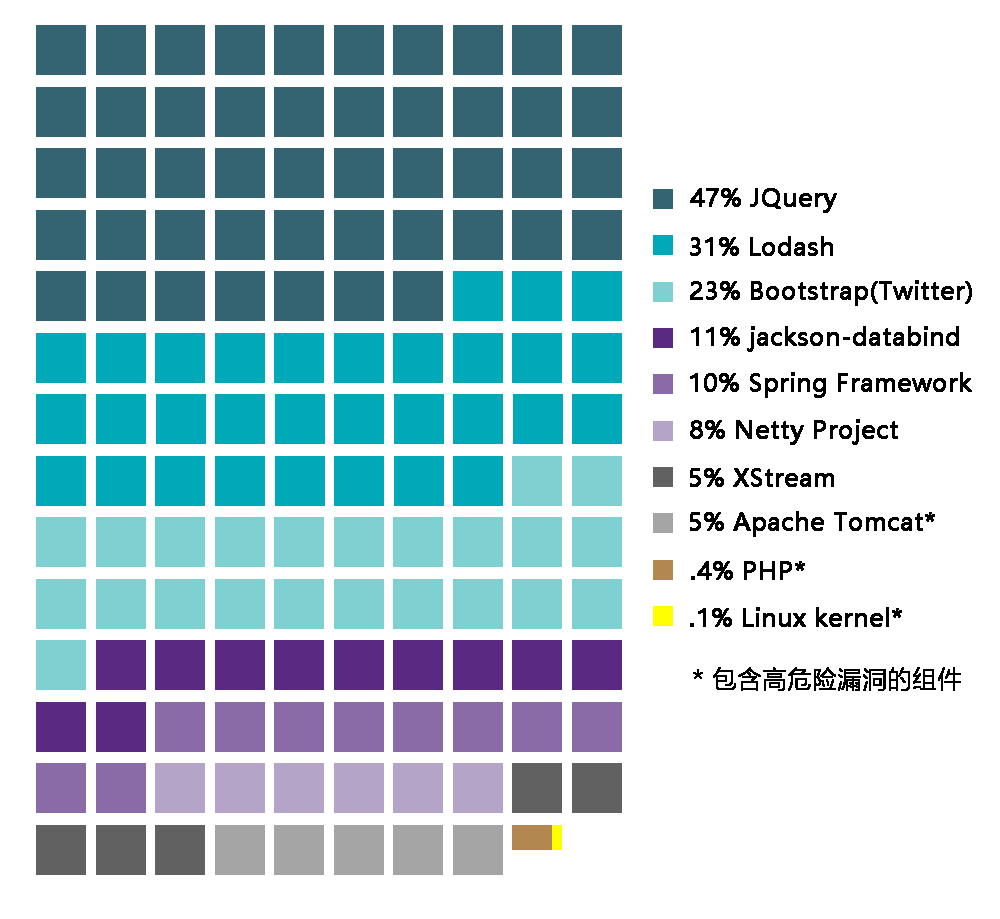
\includegraphics[width=0.75\textwidth]{figures/assembly}
    \caption{2022年Synopsys审计代码库中包含易受攻击组件的百分比示意图}
    \label{fig:assembly}
\end{figure}

早期进行代码克隆检测通常采用人工检查并标注的方法,通过收集整理大量的代码逐行检查语法、语义结构,由人工复查筛选出正确的克隆代码并对其进行标注,由此形成了早期的代码克隆数据样本,例如,2015年Svajlenko\cite{7332459}等人提出了著名评估基准集BigcloneBench,该数据集是由克隆领域三个专家评委花费216小时通过人工验证的方法从IJaDataset\cite{IJaDataset2.0}中挖掘而来,总数据量达到800万,其背后的人工花费巨大。但利用人工的方法检测代码克隆效率低,成本高,并且无法保证准确率\cite{7965429},因此,有研究人员提出代码克隆检测技术,目的在于自动化定位软件系统中的代码克隆,并能够节约成本,减少出错风险\cite{Yang2015ClassificationMF}。

早期代码克隆检测技术通常将代码视为自然语言文本进行处理,通过文本相似性判断代码相似程度;随着编译技术的发展,研究者们将编译原理中的词法分析技术运用到代码克隆检测领域;近年来,基于多维源代码表征学习的代码克隆检测技术已经引起了学者们广泛的兴趣,有研究人员从代码克隆检测与代码表征学习技术相结合这一方面进行了探索,试图从关键技术点入手,找到合适的结合点,以提高定代码克隆检测技术的效率和智能化程度。


\section{研究现状与趋势}

\subsection{代码克隆检测技术}
%\label{sec:features}
代码克隆检测技术,旨在自动化定位软件系统中的代码克隆,节省成本,减少出错风险,有助于更好地保证软件质量。目前已有的代码克隆方法大多需要对代码片段进行信息抽取,转换为中间表征,然后根据表征方式的不同计算不同代码片段之间的相似度,完成克隆检测任务。其具体流程如图\ref{fig:figure1}所示。
\begin{figure}[H]
    \centering
    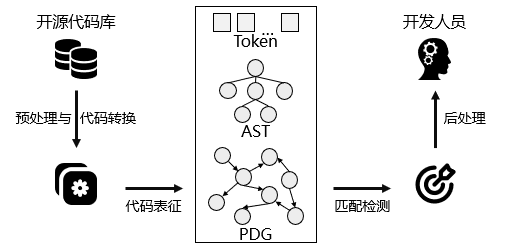
\includegraphics[width=0.95\textwidth]{figures/figure1}
    \caption{代码克隆检测流程}\label{fig:figure1}
\end{figure}

从图\ref{fig:figure1}可以看出一个完整的代码克隆检测过程通常包括预处理与转换、代码表征、匹配检测、后处理几个阶段。具体而言,一般的代码克隆检测从代码预处理与转换开始,首先删除与检测无关的空白行、注释、缩进等元素,并根据检测粒度将源代码划分为单独的片段,比如类、函数等;然后在代码表征步骤,将比较单元转换为相应的中间表示,常见的中间表示有:词法单元(Token)、抽象语法树(abstract syntax tree,AST)、程序依赖图(Program dependency graph,PDG)等;在匹配检测阶段,将根据得到不同的中间表示采用相应的匹配算法进行相似度计算,例如抽象语法树的比较通常采用子树匹配算法,程序依赖图的比较则采用子图同构算法。此阶段将代码片段两两对比,以查找相似代码源片段,得到代码克隆对。最后在后处理阶段,通常会通过人工检测或者算法过滤掉错误的代码克隆,并以适当的方式呈现给开发人员提供帮助。

在这些步骤中,代码表征方式决定了匹配检测方法的预处理方式、模型设计、部署方式、运行效率,并影响最终结果\cite{陈秋远2019代码克隆检测研究进展}。比如将源代码表征为文本,其预处理过程主要为去除噪声,如空格、注释等,其比较算法可以利用文本相似的一系列方法,能够检测到语法相似的克隆代码;而如果表征为抽象语法树,则其预处理过程需要解释器的参与,相似比较算法更多地考虑了结构相似等,能够检测到语法层面相似的代码克隆。因此, 源代码表征方式是代码克隆检测的关键步骤。

\subsection{代码表征学习}

代码表征是对代码数值化的一种技术,把代码映射为一组连续的实值向量,提取隐藏在代码内部的属性,辅助程序员生成或分析代码,是代码克隆、代码推荐、代码剽窃等软件工程任务的核心技术和研究热点\cite{谢春丽_53}。代码表征学习是指利用机器学习或深度学习技术从源代码中学习有效的表示,以便于后续的代码克隆检测等软件工程任务。在代码克隆检测中,代码表征学习可以用来提取代码片段更高层次的抽象特征表示,这些特征表示能够捕捉代码的语法、语义以及结构信息。通过学习到的代码表征,可以更准确地比较和识别不同代码片段之间的相似性,从而实现克隆代码的检测和管理,提高检测的准确性和鲁棒性。因此,代码表征学习为代码克隆检测提供了重要的技术支持,从而更有效地利用机器学习和深度学习技术来处理大规模的代码库,并提高代码克隆检测的性能和效率。

代码表征学习工作最早可追溯到100年前,基于传统机器学习的数据特征学习被广泛提出。1901年,K.Pearson提出最著名的主成分分析(Principal Component Analysis,PCA)方法\cite{WOS:000202849800065},即通过一个线性映射学习复杂高维数据的低维表示。1936年线性判别分析(Linear Discriminant Analysis,LDA)被Ronald A. Fisher提出\cite{2012THE},这是经典的有监督的表征学习方法,Fisher判别准则也由此而来。随着代码表征学习工作的不断发展,神经网络逐渐被用于特征学习,但直到1986年,Geoffrey Hinton\cite{1986Learning}发现反向传播算法(BP Algorithm)可以在网络的隐藏层里学习到有用的关于输入数据的内在表征。2006年,Geoffrey Hinton提出贪婪分层预训练和深度神经网络微调\cite{2006A}的方法,从而解决了困扰神经网络用于特征学习的两大难题:模型过拟合(Model Overfitting)和梯度扩散(Gradient Diffusion)。随着计算机计算能力的提升和深度神经网络结构的不断发展,人们更多地使用深度神经网络来更有效地提取数据的特征,用于后续的分类或预测。2013年,Y Bengio等人发表了关于表征学习的经典综述\cite{Bengio2013Representation}。2016年,Bengio和 IGoodfellow等人合著的《Deep Leanring》一书中也为表征学习专著一章\cite{goodfellow2016deep}。

近些年来,源代码表征学习方法被用于代码克隆检测、代码推荐、代码剽窃等多个代码分析任务中,取得了一定的成就。根据源代码的抽象层次不同,现阶段代码表征学习工作可以分为基于Token的代码表征、基于树的代码表征、基于图的代码表征、基于语法和语义混合的代码表征四类。

(1)基于Token的代码表征

基于Token的代码表征通常利用词法分析器将代码中的词汇单元(Token)划分出来。这些词汇单元通常包含关键字、数字、标识符等。将代码表示为词汇单元序列之后,利用深度学习技术对其进行建模,学习代码序列中所包含的有效信息,如功能语义信息、语法结构信息等,最后生成具有丰富代码信息的表征向量,应用于后续的代码克隆检测任务中。

著名的CCFinder\cite{1019480}、CP-Miner\cite{1610609}等克隆检测工具都是基于Token级的,可以很好地检测完全相同的代码对以及参数化后的代码对克隆问题。其中,CCFinder将源代码中的每一行单独转换为Token序列,根据转化规则对Token进行修改,将类型名、变量名、常量的标识符替换为指定的特殊Token,最后利用后缀树匹配算法来查找代码克隆。CP Miner增加了Bug检测,该工具的检测速度、检测精度相较于CCFinder有了很大的提高。

CCLearner\cite{10.1145/1287624.1287634}是第一个使用神经网络在Token级别进行代码克隆检测的方法,它使用BigCloneBench\cite{7332459}作为训练样本,抽取了其中方法级别的Token序列,从已有的标记数据集对DNN模型进行训练,学习保留字、类型标识符、方法标识符和变量标识符等八个特征并用于代码克隆检测。

Mikolov等\cite{pennington-etal-2014-glove}利用Word2vec、GloVe、BERT进行Token 的预训练,通过无标注样本训练深度网络结构,使用标注样本进行模型参数微调,从而提升模型性能。其中BERT\cite{devlin-etal-2019-bert}是双向Transformer的编码器,通过遮蔽语言模型和下一句预测2种预训练目标来调整模型参数。

Feng等\cite{Feng2020CodeBERTAP}提出多模态的预训练模型,利用不同模态的信息互补作用,有效提升了模型的整体表征能力。CodeBERT基于文档和代码,在自然语言和程序语言双模态下,利用BERT进行预训练,提取自然语言和程序语言之间的语义连接,为下游任务提供通用表示向量。

上述方法均在Token上进行代码的表征学习,力图充分提取代码中的属性信息。

(2)基于树的代码表征

抽象语法树AST是源代码的抽象语法结构的树状表示,可以有效地表示程序的语法及其结构,利用深度神经网络对抽象语法树进行建模得到其向量表示,根据该特征向量完成代码克隆检测任务,实现基于树的源代码表征。

White等人\cite{White2016DeepLC}提出了一种基于循环神经网络的代码表征方法,该方法将代码分为词汇以及句法两个层次。对于词汇级别的信息,该方法在代码的词汇单元序列上使用 RNN神经网络进行建模。而对于代码的句法级别的信息,首先将代码转换为其对应的抽象语法树结构,之后将抽象语法树转换为其对应的满二叉树,最后将满二叉树转换为橄榄树,并在其上使用另一个RNN神经网络进行建模。该方法将这两个特征相结合作为整个程序的特征向量,根据该向量进行代码克隆检测任务。

Mou等人\cite{WOS:000485474201046}提出了一种基于树的卷积神经网络模型(tree-based convolutional neural network,TBCNN)。该模型采用了“连续二叉树”的概念,直接在代码所对应的抽象语法树上进行卷积操作。在卷积操作之后获得了不同数目的AST结构特征向量,由于数目不同不能直接作为神经网络的输入,因此该方法还采用“动态池化”技术,最终将数目不同的特征向量转换为了一个向量。TBCNN是一个通用的代码表征生成模型,所生成的向量能够包含代码片段中特有的代码模式,因而可以应用于不同的代码分析任务中。

Wei等人\cite{10.5555/3172077.3172312}提出了CDLH(Clone Detection with Learning to Hash)方法,该方法在抽象语法树的基础上使用LSTM模型,通过共享权重的方式学习两个代码片段之间的表征向量,然后利用特定哈希函数来将其编码为二进制哈希码,最后工具通过计算哈希码的汉明距离来检测代码克隆。

Chen等人\cite{10.1145/3310273.3321560}采用了基于树的卷积神经网络,该方法考虑到已有的方法仅仅使用抽象语法树会造成代码语义信息的丢失,因此该方法将API的调用信息作为补充信息合并到抽象语法树中,之后进行代码表征。在POJ104\cite{WOS:000485474201046}和BigcloneBench\cite{7332459}数据集上进行实验,在F1指标上获得了0.39和0.12的提升。

Zhang等人\cite{8812062}提出了一种基于抽象语法树的神经网络代码表征方法,该方法将代码转换为其对应的抽象语法树,然后将完整的抽象语法树分割为多个语句树。针对每个语句树,该方法设计了语句编码器用于将语句树转换为对应的语句表征向量,通过使用双向GRU神经网络对语句向量进行建模,对双向GRU层输出的隐含状态向量进行最大池化操作,以获得最显著的代码特征。该方法所生成的代码表征向量被应用于代码克隆检测任务中,在POJ104\cite{WOS:000485474201046}和BigcloneBench\cite{7332459}数据集上取得了当时最好的检测结果。

上述方法均在抽象语法树上进行代码的表征学习,力图充分提取代码中的结构信息。

(3)基于图的代码表征

程序依赖图PDG是程序的一种图形表示,所含结构信息最多,能够表示程序的控制依赖,数据依赖以及地址依赖等关系,是一种带有标记的有向多重图。通过将程序表示为图的形式使得模型能够更好地理解代码中不同部分之间的依赖关系。

Allamanis等人\cite{Allamanis2017LearningTR}考虑到代码中的长依赖问题,如在代码中变量的定义位置与使用位置之间的距离问题,提出了基于图的代码表征方法,旨在学习代码中的语法以及语义结构。首先将代码转换为对应的抽象语法树,之后通过不同的连接规则连接抽象语法树各个节点,获得了包含变量之间依赖关系在内的不同节点之间的关联关系;最后将构建好的代码图数据作为输入,输入到图神经网络中进行表征学习。

Lu等人\cite{Lu2019ProgramCU}从代码中提取数据流与函数调用信息,将其融合到抽象语法树中,从而将代码构建为一个包含丰富信息的图结构表示。在传统的GGNN模型上引入了注意力机制,用于获得图中每个节点的重要程度,进而获得更具有区分度的代码表征向量。

Brockschmidt等人\cite{Brockschmidt2018GenerativeCM}同样在代码的抽象语法树上增加相应的边以构建代码图,代码图的构建方法与文献\cite{Allamanis2017LearningTR}类似。之后采用图神经网络对程序的结构和数据流进行建模完成代码表征任务。

Ben-Nun等人\cite{10.5555/3327144.3327276}提出了一种与语言以及平台无关的代码表征方法inst2vec。该方法首先使用编译器对代码进行编译,得到代码的中间表示。但由于该中间表示并没有包含代码之中的数据流信息以及控制流信息,因此该方法将数据流和控制流也融合到该中间表示中,进而构建了代码上下文流图。最后在所构建的图上使用循环神经网络进行建模,获得代码的表征向量。该向量在程序分类实验中的准确率取得了当时最好的效果。

Wang等人\cite{9054857}考虑了仅仅使用代码的抽象语法树进行代码表征建模实际上仍然有代码结构上的缺失这一问题,构建了代码抽象语法树的图形表示FA-AST,通过将抽象语法树各个叶子结点相连构建出适合图神经网络处理的数据,然后应用两种不同类型的图神经网络GNN来检测克隆。

DeFreez等人\cite{10.1145/3236024.3236059}提出了Fun2Vec方法,解决代码的路径爆炸问题,该方法采用随机游走算法,随机选择部分执行路径,捕获程序的层级结构,每条执行路径转换为一个标签序列,借助Word2Vec方法,把标签映射为连续实值向量,并通过神经网络训练函数的嵌入向量。

Duan等人\cite{WOS:000680742600067}提出了一种无监督的程序代码表示学习技术DEEPBINDIFF,依靠代码语义信息和程序控制流信息生成基本块嵌入,并且采用k-HOP贪婪匹配算法利用基本块嵌入发现最优的相似性结果。通过大量二进制文件和真实的OpenSSL漏洞对原型进行评估,结果表明DEEPBINDIFF相比于最先进的工具,跨版本和交叉优化级别都更优。

Kang等人\cite{Yang2021AGS}提出了一种基于门控神经网络的CC-GGNN方法来解决代码补全问题。CC-GGNN通过从代码表示中获得有效的代码特征,提出了一种分类机制,通过使用已知的父节点对节点的表示进行分类,并在模型中构建训练图。实验结果表明,模型在数据集中最多优于最先进的方法MRR最多9.2\%,ACC最多11.4\%。

上述方法均在图上进行代码的表征学习,力图充分提取代码中的语义信息。

(4)基于语法和语义融合的代码表征

基于语法与语义融合的模型,结合AST、DFG、CFG、Token序列,捕获程序的语法及语义结构信息。其中抽象语法树AST和Token序列反映了语法层面的信息,DFG、CFG反映了语义层面的信息。

Tufano等人\cite{Tufano2018DeepLS}采用四种不同的代码表征方法(即标识符、抽象语法树、字节码和CFG)进行代码克隆检测,他们利用四种代码表示分别识别代码对的相似度,并计算平均值作为最终的相似度结果。

Fang等人\cite{Fang2020FunctionalCC}结合抽象语法树,控制流图和调用图来学习代码特征,融合了语法和语义信息。首先,该方法从源码中分析出方法之间的调用图、每个方法的抽象语法树以及每个方法的控制流图;然后,用调用图将找出每个功能的AST集合。通过AST集合抽取功能的语法信息;通过调用图组成每个功能的控制流图;通过控制流图抽取功能的语义信息;最后,将抽取出来的语义信息送入前馈神经网络得到分类结果。

Hua等人\cite{Hua2020FCCAHC}结合标记、抽象语法树和控制流图三种方式实现检测目标。文中提出了使用注意力的代码克隆检测器(FCCA),这是一种基于深度学习的代码克隆检测方法,它通过保留多个代码特征,包括非结构化(以顺序令牌形式的代码)和结构化(以抽象语法树和控制流图形式的代码)信息,在混合代码表示的基础上进行代码克隆检测。将多个代码特征融合到混合表示中,该混合表示配备有注意力机制,有助于最终检测精度的重要代码部分和特征。

Dong等人\cite{9148302}提出了一种基于Token和AST的代码表征方式,提取数量特征如AST中的AST树的高度、节点数以及标记中操作数的个数、字符串的个数等作为神经网络的输入进行检测。

亚芳等人\cite{王亚芳2020基于图像相似度检测代码克隆}提出了一种基于图像相似度的代码克隆检测技术。该方法区别于传统方式,从图像处理角度提出了一种基于图像相似度的新型代码克隆检测(CCIS)方法。首先对源代码进行移除注释、空白符等操作,以获取"干净"的函数片段,并将函数中的标识符、关键字等进行高亮处理;然后将处理好的源代码转换为图像,并对图像进行规范化处理;最后使用Jaccard距离和感知哈希算法进行检测,得到代码克隆信息。

Saini等人\cite{10.1145/3236024.3236026}提出了一种代码克隆检测框架Oreo,该方法从程序的源代码中提取了包括被调用的外部方法的数量、变量的数量、语句的数量、循环的数量等24种度量,然后进一步从函数中抽取语义,并使用了基于哈希的方法进一步筛选,最后加入了深度学习的方法,将两个程序向量输入到孪生模型中来判断两个程序之间是否具有克隆关系。

SrcClone\cite{ALOMARI2022111115}是一种基于切片的克隆检测方法,主要用于检测语法和语义代码克隆,该方法使用了轻量级、公开可用、可扩展的程序切片器。具体来说,SrcClone使用切片信息计算基于切片的指标,这些指标可以用来计算某些切片向量以近似切片内部的结构信息,然后在定制的局部敏感哈希算法中使用这些信息来有效地散列和聚类相似的向量。如果两个代码片段对应的片段也相似,则 srcClone认为它们在语义上相似。这些类似的切片表示候选克隆类。

总体而言,代码克隆检测是软件工程领域一项重要任务,如何对代码进行合适的表征是代码克隆检测的关键问题。代码表征学习决定了对源代码信息抽取程度的上限,决定了检测技术的预处理方法、模型设计、部署方式、运行效率,并会影响最终结果。面向代码克隆检测这一下游任务,代码表征学习研究存在以下不足:对代码结构信息语义信息利用不充分,特征表达不够完善;表征模型对数据集、模型结构和优化算法等多方面因素的要求高等问题,这些不足严重制约着代码克隆检测技术的发展。因此,研究人员一方面通过对源代码进行充分利用,提出多维源代码表征方法,从而提高代码克隆检测能力;另一方面,通过研究更先进的算法来提高表征模型的自动化和智能化程度,也是目前重要的发展趋势。

\section{研究内容}
本文主要围绕如何将源代码表征学习技术应用到代码克隆检测领域,通过不同维度对程序表征进行学习,并基于学习得到的语义特征进行克隆对的判定,充分发挥代码表征学习技术检测代码克隆的能力。针对现有代码表征学习方法存在的对代码结构信息和语义信息利用不充分的问题,本文提出面向代码克隆检测的多维源代码表征学习方法RLCCD ,旨在通过构建三个不同维度的代码表征模型,将源代码的语义信息表示为稠密低维实值向量,以在低维空间中高效计算实体和关系的语义联系,并通过特征融合得到多维特征,实现对代码信息的充分利用,以更加全面准确与智能化的方式提高代码克隆测试效率。

本文的主要工作包括:

(1)提出面向代码克隆检测的多维源代码表征学习方法RLCCD 

本文提出了一种面向代码克隆检测的多维源代码表征学习方法RLCCD,该框架主要针对代码表征关键步骤提出三个关键技术点,从Token序列、抽象语法树AST、程序依赖图PDG三种不同维度对代码特征表示进行优化,分别形成了基于预训练辅助模型的Token表征学习、基于子树划分的抽象语法树表征学习、基于图过滤的程序依赖图表征学习三种方法,然后通过特征融合将三种维度特征整合为一个多维特征,实现对代码信息的充分利用,以更加全面准确与智能化的方式提高代码克隆测试效率。 

(2)基于预训练辅助模型的Token表征学习

针对目前现有的基于Token的表征学习方法通常将代码表示为词汇单元,为了后续生成表征向量通常会将词汇单元规范化,丢失部分语法信息,出现在词汇表中不存在Token的难题,提出了一种基于预训练辅助模型的Token表征学习方法。该方法在模型训练之前,通过选取预训练辅助模型从代码语料库中学习基本单元的语法语义信息,以及这些单元之间的联系,最终给出一份单词-向量形式的词汇表,从而减少出现集外词问题的概率。本文在POJ104数据集上的消融实验评估表明,预训练辅助模型方法能够提高代码克隆检测准确率。

(3)基于子树划分的抽象语法树表征学习

针对现有的基于树的表征学习方法通常将抽象语法树转换为完整二叉树,可能破坏源代码原有的语法结构,增加AST高度,丢失长期上下文信息,削弱了神经模型捕捉更真实和复杂语义的能力,导致梯度消失的难题,提出了一种基于子树划分的抽象语法树表征学习方法。该方法将每个大型的AST分割成小语句树序列,并通过捕获语句的词法和句法知识将每一个语句树都编码成一个向量,在得到一个语句向量序列后,将语句向量序列输入树卷积神经网络中生成代码片段的结构向量表示。本文在POJ104数据集上的消融实验评估表明,子树划分方法能够有效提取结构特征,提高代码克隆检测准确率。

(4)基于图过滤的程序依赖图表征学习

针对现有的基于图的表征学习方法通常将程序表征为有向多重图,继而采用图匹配算法将图中的控制流和数据流编码为一个紧凑的语义特征矩阵,矩阵中每个元素都是高维系数特征向量,所消耗的时间、空间开销巨大的难题,提出了一种基于图过滤的程序依赖图表征学学习方法。该方法通过收集PDG的简单特征来过滤掉明显不可能为克隆的PDG对。具体的,根据PDG的节点个数、控制边数、执行边数、数据边数、声明节点数、函数调用数、传入参数、传出参数等代表特征进行过滤,在大幅减少候选PDG对规模的同时,保证真正的克隆对不会被过滤掉而导致整体克隆检出率的降低。本文在POJ104数据集上的消融实验评估表明,图过滤方法能够有效减少时间、空间开销,提高代码克隆检测准确率。

(5)特征融合及实验验证

针对不同的特征采用不同的代码表征模型对代码片段进行多维源代码特征学习,从而提高对源代码特征提取的程度,并通过特征融合得到一个更能代表代码信息的多维特征,该多维特征能够在低维空间中高效计算实体和关系的语义联系,提高后续代码克隆检测任务的准确率。

本文选取了代码克隆检测领域常见的基准集POJ104进行实验验证,并与现有开源的SourcererCC\cite{7886988}、ASTNN\cite{8812062}、SCDetector\cite{10.1145/3324884.3416562}方法进行比较,主要通过召回率(Recall)、精确度(Precision)和准确率(Accuracy)三个指标评价实验结果,实验结果验证了RLCCD的可行性和有效性。

\section{论文结构}
%\label{sec:requirements}
本文共由6章组成,具体的组织结构如下:

\textbf{第1章} \quad 绪论部分首先对本文的研究背景与意义进行了阐述,并对代码克隆检测技术和代码表征学习技术的研究现状与趋势进行了分析总结,进而提出本文的主要研究内容,最后对全文的组织结构进行了介绍。

\textbf{第2章}  \quad 分析了代码表征学习领域的关键技术挑战,基于此,提出了本文的面向代码克隆检测的多维源代码表征学习方法RLCCD,并对该技术的整体框架进行了介绍,进而根据所提框架简要论述了本文研究的关键技术,即基于预训练辅助模型的Token表征学习方法、基于子树划分的抽象语法树表征学习方法、基于图过滤的程序依赖图表征学习方法。

\textbf{第3章}  \quad 介绍基于预训练辅助模型的Token表征学习方法的设计与实现。首先,分析其研究动机,即目前Token表征学习面临的集外词问题,继而提出基于预训练辅助模型的方法设计,详细介绍该方法的设计思路和具体实现,最后,对该方法的有效性进行消融实验验证。

\textbf{第4章}  \quad 介绍基于子树划分的抽象语法树表征学习方法设计与实现。首先,分析其研究动机,即目前抽象语法树表征学习面临的梯度消失问题,继而提出基于子树划分的方法设计,详细介绍该方法的设计思路和具体实现,最后,对该方法的有效性进行消融实验验证。

\textbf{第5章}  \quad 介绍基于图过滤的程序依赖图表征学习方法设计与实现。首先,分析其研究动机,即目前图表征学习面临的计算开销大问题,继而提出基于图过滤机制的方法设计,详细介绍该方法的设计思路和具体实现,并给出了针对该方法有效性的消融实验验证。

\textbf{第6章}  \quad 介绍特征融合及本文研究框架RLCCD的实验验证。首先,针对特征融合的方法设计与具体实现进行了介绍。接着,对RLCCD框架的有效性进行了评估,通过与现有开源技术SourcererCC、ASTNN、SCDetector进行实验对比,验证RLCCD方法的有效性。

\textbf{结论}  \quad 对全文的研究进行了总结,并提出对未来工作的展望。